\documentclass[a4paper,cleardoubleempty,BCOR1cm]{scrbook}
% use to waste space:
% \documentclass[12pt,a4paper]{article}

% if you have this style and like it.
%\documentclass{acmsiggraph}
%\documentclass[review]{acmsiggraph}      % review
%\documentclass[widereview]{acmsiggraph}  % wide-spaced review
%\documentclass[preprint]{acmsiggraph}    % preprint

% define a \comment{this is a comment which can have linebreaks in it}
\newcommand{\comment}[1]{}
% \newcommand{\todo}[1]{\marginpar{\bf{#1}}}
\newcommand{\todo}[1]{{\color{red}\bf{TODO: #1}}}

\usepackage{mathptmx}
\usepackage[pdftex]{graphicx}
\usepackage[pdftex]{color}
\definecolor{rot}{RGB}{165,30,55} %rote Farbe
\graphicspath{{./images/}}
\usepackage{parskip}
\usepackage{amsmath}
% \usepackage{dsfont}
\usepackage{pxfonts}

\usepackage[T1]{fontenc}
\usepackage{textcomp}

% comment these two lines out if you don't want minion/myriad fonts.
% \usepackage[minionint,mathlf]{MinionPro}
% \renewcommand{\sfdefault}{Myriad-LF}
%\usepackage{Myriad}

% no page number on float pages, fixes problems with overlarge diagrams.
\usepackage{fancyhdr}
\pagestyle{fancy}
%\lhead{}
%\chead{}
%\rhead{}
%\lfoot{}
\fancyhf{}
\fancyhead[EL]{\nouppercase{\leftmark}}
\fancyhead[OR]{\nouppercase{\rightmark}}
\cfoot{}
%\fancyfoot[EL]{\iffloatpage{}{\thepage}}
%\fancyfoot[OR]{\iffloatpage{}{\thepage}}
\fancyfoot[EL]{\thepage}
\fancyfoot[OR]{\thepage}
\renewcommand{\headrulewidth}{0pt}
\renewcommand{\footrulewidth}{0pt}

%\usepackage{natbib}		% textual referencing
%\usepackage[numbers,super]{natbib}	% nice superscripts
%\bibliographystyle{chicago}	% shitty
\bibliographystyle{alpha}	% abbr names and year in \cite
%\bibliographystyle{agsm}	% australian, need natbib
%\bibliographystyle{kluwer}	% need natbib
%\bibliographystyle{apalike}	% lengthly
%\bibliographystyle{abbrv}	% minimal?

% use for german line breaking:
%\usepackage[ngerman]{babel}
\usepackage[T1]{fontenc}
\usepackage[utf8x]{inputenc}

% avoid us-style text color destruction:
\frenchspacing
\usepackage{microtype}

% have a nice framebox with border directly around the image:
\fboxsep 0pt
\newcommand{\fimg}[2]{\fbox{\includegraphics[width=#1]{#2}}}

\usepackage{theorem}
\theorembodyfont{\upshape}
\newtheorem{definition}{Definition}

\usepackage{listings}
\lstset{numbers=left, numberstyle=\tiny, basicstyle=\tiny, language=C++}
\usepackage[boxruled]{algorithm2e}
%\usepackage{hyperref}
\usepackage{url}
\usepackage{subfig}

\def\code#1{{\tt{#1}}}



\title{Thesis Template}
\author{Peter Trost\thanks{e-mail: peter.trost@student.uni-tuebingen.de}}
\date{\today}
\begin{document}

\begin{tabular}{lr}
% 
\includegraphics[width=0.5\linewidth]{logo_sw} % logo bw
 
\includegraphics[width=0.5\linewidth]{UT_WBMW_Rot_4C} % logo red
 & \hspace{0.2\linewidth}
 \parbox{0.5\linewidth}{
   \large\bf\textsf{\color{rot}{Mathematisch-\\Naturwissenschaftliche\\Fakultät\\\\}}
  \hspace{-.144cm}\normalsize\textsf{\color{rot}{Lernbasierte Computer Vision}}
   \vspace{0.6cm}
 }
\end{tabular}

\vspace*{10ex}
Bachelorarbeit

{\huge\bf\textsf{A Comparison of Synthetic-to-Real Domain Adaptation Techniques}}

\vspace*{30ex}

Eberhard Karls Universität Tübingen\\
Mathematisch-Naturwissenschaftliche Fakultät\\
Wilhelm-Schickard-Institut für Informatik\\
Lernbasierte Computer Vision\\
Peter Trost,~ \verb+peter.trost@student.uni-tuebingen.de+,~ 2019

\vspace*{5ex}

\begin{tabular}{@{}l@{\hspace{2em}}l}
  Bearbeitungszeitraum:& 24.05.2019-23.09.2019 \vspace*{5ex} \\
  Betreuer/Gutachter:& Prof. Dr. Andreas Geiger, Universität Tübingen\\
  					 &Despoina Paschalidou, ETH Zürich\\
  					 &Dr. Yiyi Liao, Max-Planck-Institut für Intelligente Systeme Tübingen
\end{tabular}

\thispagestyle{empty}
\newpage

\chapter*{Selbstst\"andigkeitserkl\"arung}
Hiermit versichere ich, dass ich die vorliegende Bachelorarbeit selbst\"andig und
nur mit den angegebenen Hilfsmitteln angefertigt habe und dass alle Stellen,
die dem Wortlaut oder dem Sinne nach anderen Werken entnommen sind,
durch Angaben von Quellen als Entlehnung kenntlich gemacht worden sind.
Diese Bachelorarbeit wurde in gleicher oder \"ahnlicher Form in keinem anderen
Studiengang als Pr\"ufungsleistung vorgelegt.

\vspace*{8ex}
\hrule
\vspace*{2ex}
Peter Trost (Matrikelnummer 4039682), \today



\chapter*{Abstract}
Template

\chapter*{Acknowledgments}
If you have someone to Acknowledge ;)

\tableofcontents

%% braucht kein Mensch ...
%\listoffigures
%\listoftables

% write content here or...
\chapter{Introduction}
What is this all about?

Cite like this: \cite{agarwal2011}

\chapter{Related Work}
\section{Synthetically rendered datasets}
\subsection{A naturalistic open source movie for optical flow evaluation}
\cite{Butler:ECCV:2012}

\begin{figure}[h]
	\centering
	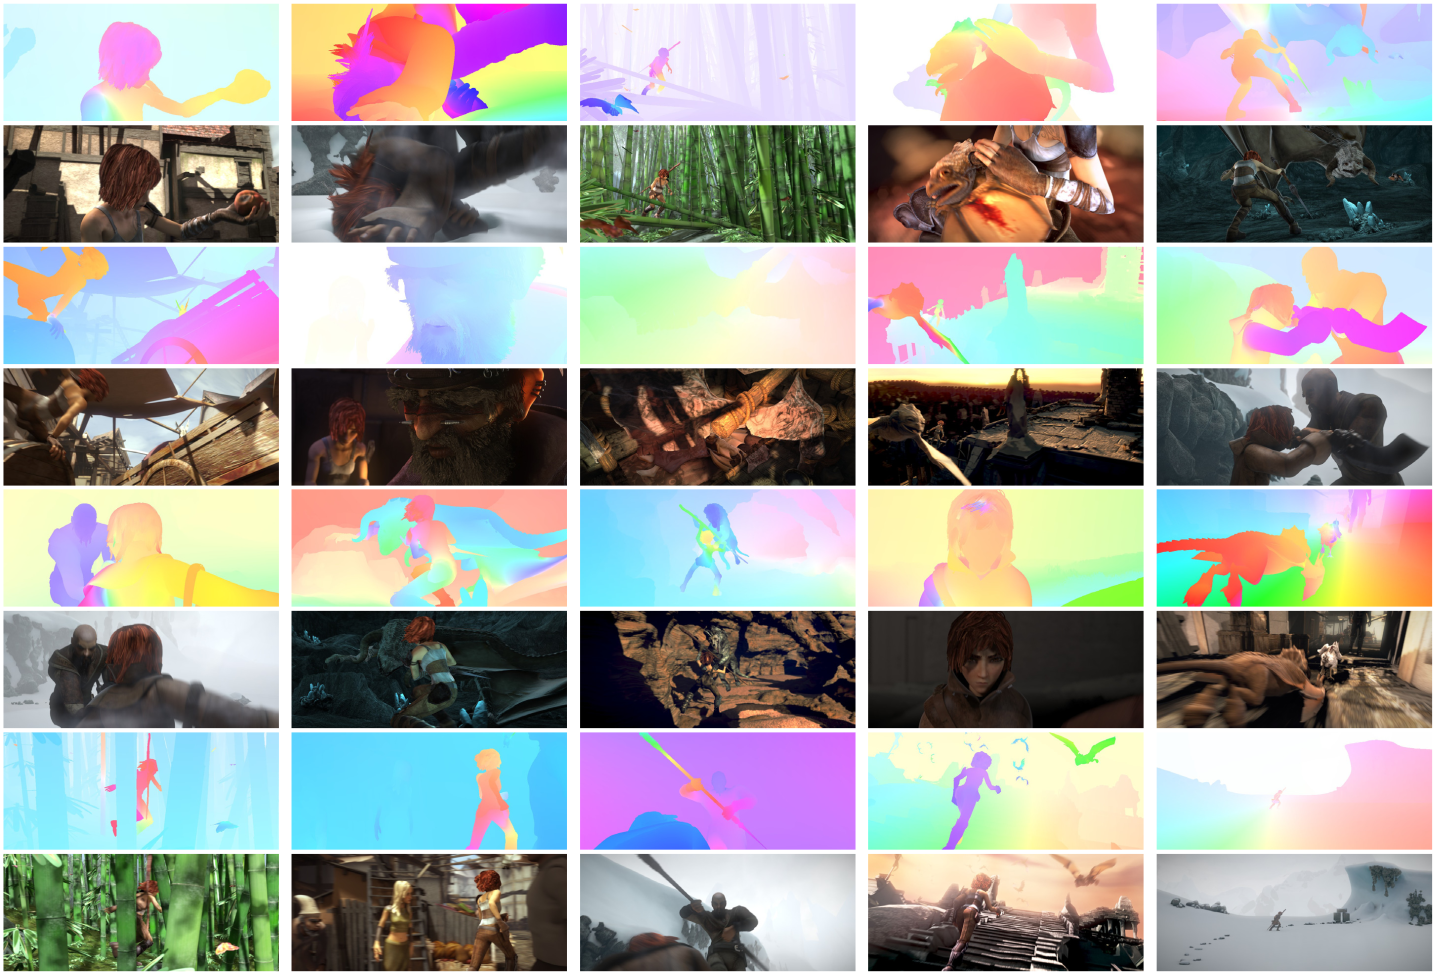
\includegraphics[width=\textwidth]{images/Sintel.png}
	\caption{Example images (ground truth flow in uneven rows and RGB in even ones) from the Sintel dataset}
	\label{Sintel}
\end{figure}



\subsubsection{Overview}
In this paper the authors provide a dataset for optical flow estimation derived from the open source 3D animated short film Sintel
\todo{cite Sintel: https://durian.blender.org/}.
The dataset contains long sequences, large motions, specular reflections, motion blur, defocus blur, atmospheric effects and more. Its scenes are rendered in varying complexity through the source graphics data provided by the authors of the film. Because of this aforementioned variety the dataset can be used to improve optical flow methods. 

\subsubsection{Render passes}
As mentioned above the dataset contains image sequences rendered in the following variying complexity:\\
\begin{itemize}
	\item Albedo Pass: Flat and unshaded. Surfaces exhibit constant albedo over time
	\item Clean Pass: Illumination including smooth shading and specular reflections adds realism
	\item Final Pass: Full rendering with all effects including blur due to camera depth of field and motion, and atmospheric effects.
\end{itemize}

\subsubsection{Main aspects}
The main aspects of the Sintel dataset are the following:\\
It contains varying and more challenging (for existing methods) scenes than older datasets. Sequences are 50 frames long and are provided with 49 ground truth flow fields which are a measure of changes in position for objects in the scene from frame to frame. Some frames include motions of well over 100 pixels. There are 1628 frames with 564 for testing and 1064 for training. The Sintel dataset contains sequences having real-world challenges like lighting variations, shadows, complex materials, reflections and more.

\subsubsection{Meta}
The authors modified Blender's internal motion blur pipeline to give accurate motion vectors at each pixel which provide ground truth optical flow maps. Although the clips are selected so that optical flow is realistic, one still has to be cautios when training and evaluating algorithms that strongly rely on real-world laws of physics. The images are saved as 8-bit PNG files and the clips have a framerate of 24 fps.

\newpage

\subsection{Playing for data: Ground truth from computer games}
\cite{Richter_2016_ECCV}

\begin{figure}[h]
	\centering
	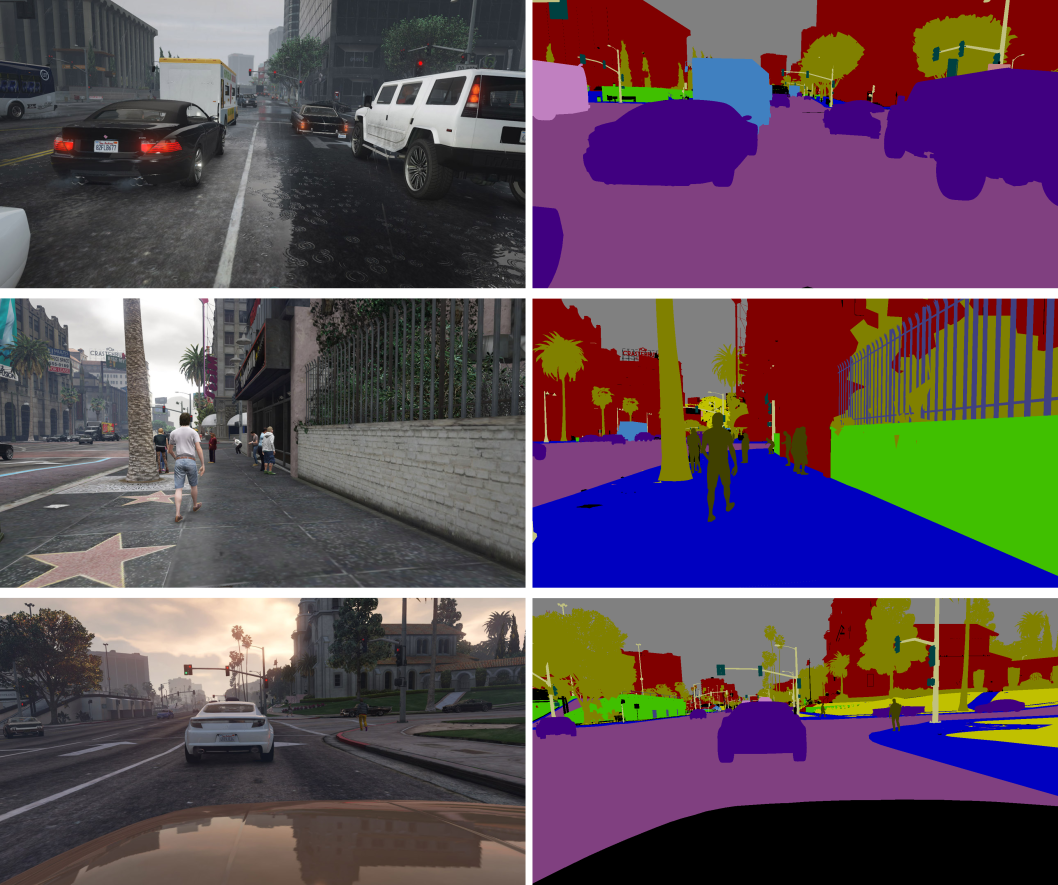
\includegraphics[width=\textwidth]{images/P4D.png}
	\caption{Example images (RGB on the left and semantic segmentation right) from the ''Playing for data``-dataset}
	\label{P4D}
\end{figure}

\section{Overview}
The main aspect of this paper is to get pixel-accurate ground truth of synthetic data and therefore be able to label objects in the images accurately and efficiently.
The authors use detouring (i.e. injecting a wrapper between the game and the operating system) to record, modify and reproduce rendering commands from the game Grand Theft Auto 5 (GTA5). They retrieve the distinct rendering resources (geometry, textures, shaders) which they hash in order to create object signatures. These signatures are then used to label the objects pixel-accurately. The signatures then enable them to propagate these labels across time and instances that share distinctive resources. The dataset of the paper contains 25,000 images from GTA5 with pixel-level semantic segmentation ground-truth. Labeling the data took 49 hours  which is 3 orders of magnitude faster than other semantic segmentation datasets with similar annotation density). This is achieved through the object signatures: When an object is labeled in a given image this label is propagated to every image that contains this object using the object signatures. 


\newpage

\subsection{The synthia dataset: A large collection of synthetic images for semantic segmentation of urban scenes}
\cite{RosCVPR16}


\newpage

\subsection{SyB3R: A Realistic Synthetic Benchmark for 3D Reconstruction from Images}
\cite{syb3r2016}







\newpage

\section{Problem Statement}
\todo{what you have to do here :)}

% ... input content via other .tex files
\chapter{Conclusion}
\label{sec:conclusion}


\section{Outlook and Future Work}

\appendix
\chapter{Blub}

\bibliographystyle{alpha}
\bibliography{bibliography}

\end{document}

